% Reachability gap: a deployed d_ff x r MLP matrix and the fraction of its
% independent output directions that LRC-style inheritance can actually train.
% Compile: pdflatex reachability_gap.tex
\documentclass[tikz,border=8pt]{standalone}
\usepackage{amsmath,amssymb}
\usepackage{xcolor}
\usetikzlibrary{arrows.meta,patterns,positioning,calc}
\begin{document}
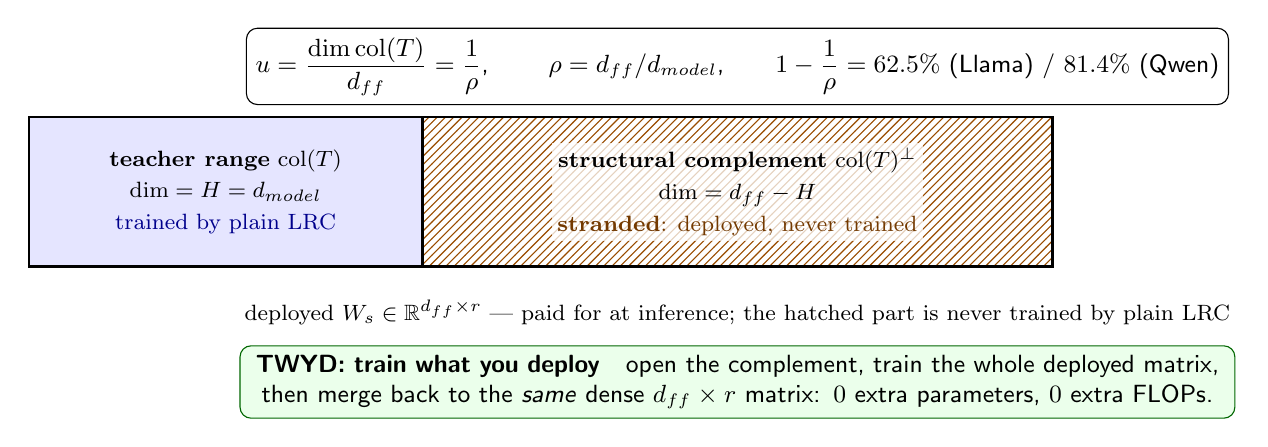
\begin{tikzpicture}[font=\sffamily\small,>=Latex]

  \def\H{5.0}          % col(W) width (proportional to H)
  \def\C{8.0}          % complement width (proportional to d_ff - H)
  \def\W{\H+\C}

  % ---- headline annotation (above the bar) -------------------------------
  \node[draw,rounded corners,fill=white,align=center,anchor=south]
       at ({\W/2},2.05)
       {$\displaystyle u=\frac{\dim\mathrm{col}(T)}{d_{ff}}=\frac{1}{\rho}$,
        \qquad $\rho=d_{ff}/d_{model}$,\qquad
        $\displaystyle 1-\frac{1}{\rho}=62.5\%\ \text{(Llama)}\ /\ 81.4\%\ \text{(Qwen)}$};

  % ---- deployed matrix, drawn as a wide bar -------------------------------
  \fill[blue!10] (0,0) rectangle (\H,1.9);
  \fill[orange!12,pattern=north east lines,pattern color=orange!60!black]
        (\H,0) rectangle (\W,1.9);

  \draw[thick] (0,0) rectangle (\W,1.9);
  \draw[thick] (\H,0) -- (\H,1.9);

  \node[align=center,font=\footnotesize] at (\H/2,0.95)
       {\textbf{teacher range} $\mathrm{col}(T)$\\[2pt]
        $\dim = H = d_{model}$\\[2pt]
        \textcolor{blue!55!black}{trained by plain LRC}};
  \node[align=center,font=\footnotesize,fill=white,fill opacity=0.75,text opacity=1,
        inner sep=2pt] at (\H+\C/2,0.95)
       {\textbf{structural complement} $\mathrm{col}(T)^{\perp}$\\[2pt]
        $\dim = d_{ff}-H$\\[2pt]
        \textcolor{orange!45!black}{\textbf{stranded}: deployed, never trained}};

  % ---- caption ------------------------------------------------------------
  \node[align=center,anchor=north,font=\footnotesize] at ({\W/2},-0.3)
       {deployed $W_s\in\mathbb{R}^{d_{ff}\times r}$ --- paid for at inference;
        the hatched part is never trained by plain LRC};

  % ---- TWYD outcome -------------------------------------------------------
  \node[draw,rounded corners,fill=green!8,draw=green!40!black,align=center,
        anchor=north,text width=12.4cm]
       at ({\W/2},-1.0)
       {\textbf{TWYD: train what you deploy}\quad
        open the complement, train the whole deployed matrix, then merge back to
        the \emph{same} dense $d_{ff}\times r$ matrix: $0$ extra parameters,
        $0$ extra FLOPs.};

\end{tikzpicture}
\end{document}

